\section{Short-Range ANT (Local)  Scouting}
\marginnote{./AE-Specifications-ETH/standalone/Scouting.tex}

Once a link has been established, they are recorded in the local \texttt{knowledge} of the cell, and used as a baseline for future algorithmic and policy decisions. 

Immediately after establishing a reliable connection, \CELLs may emit \texttt{ANT-SCOUTS} to explore their local environment. These are ANT's, which obey an initial source routing algorithm, but when encountering a failed or disconnected port in another cell, respond with either clockwise, anticlockwse packet forwarding, which keeps the scout local, or \emph{random}, with a hopcount limit, which allows exploration further afield\marginnote{See ANT Specification for details}.

\section{Long-Range BEE (Global)  Scouting}

\CELLs may also emit \texttt{BEE-SCOUTS} to explore the extremities of their environment. These are BEE's which obey only one rule: proceed in the same direction as the radial port.   BEE's  emitted on the $n$ port may only go $n$.  BEEs emitted on the $se$ port may only go $se$. Until they encounter a disconnected port, whereupon they execute a return path algorithm, accumulating information at each \CELL and returning it to the root.\marginnote{See BEE specification for details}

\section{ANT Specification: Triangle Packet Clocks in $3 \times 3$ Tiles}
 \begin{marginfigure}
        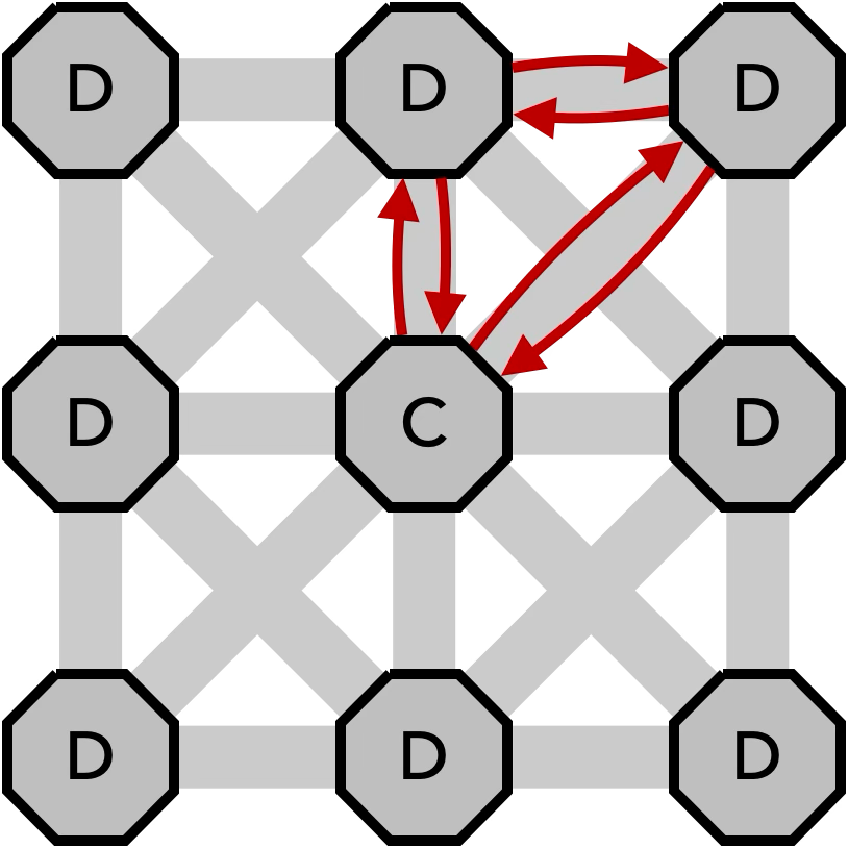
\includegraphics[width=\linewidth]{../../FIGURES/Triangle-clock.pdf} % Trim is l b r t
  \caption{Race-Free Triangle Token}
    \vspace{10pt}
\end{marginfigure}

Packet clocks are initiated by the coordinator, on any of it's active links.  The ANT (source routing) algorithm goes out on any port, and are programmed to turn left or right at the first available active port.  The convention is turning right makes it go clockwise, and turning left makes it go antilockwise, but this is an artificial distinction. As with real ants, they can get lost, and never find their way back to the nest, and they die (or return to the nest by inverting their source routing paths). This ``limited range'', is part of the Security mechanism. 

\section{ANT Specification: Race-Free Packet Clocks in $3 \times 3$ Tiles}
 \begin{marginfigure}
        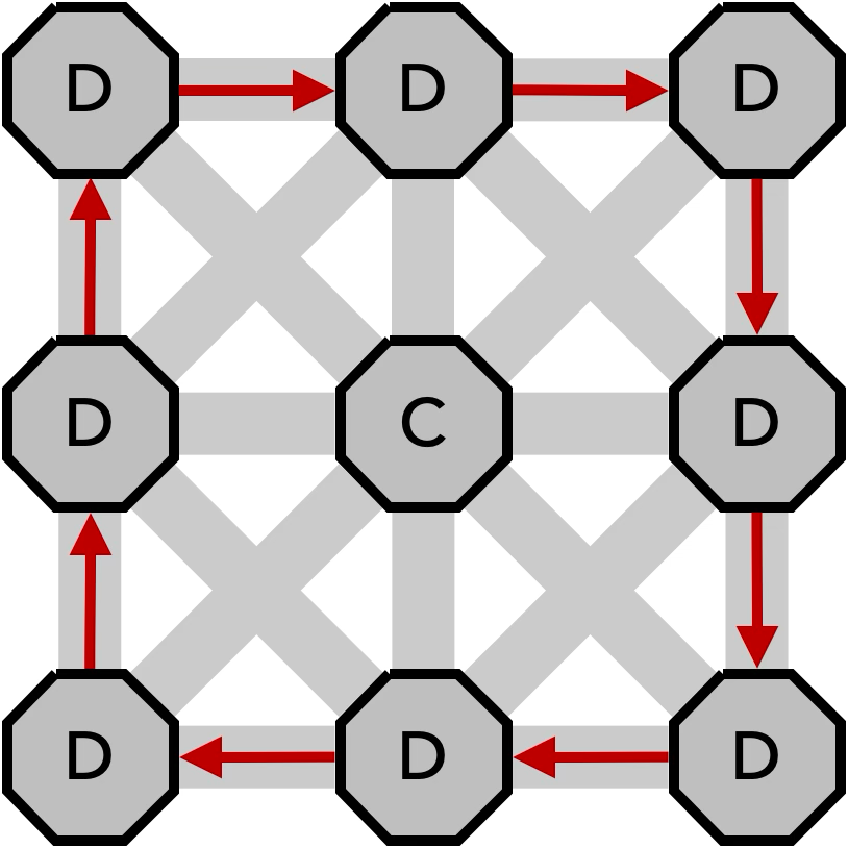
\includegraphics[width=\linewidth,trim=0mm 0mm 0mm 0mm, clip]{../../FIGURES/3x3-clockwise.pdf} % Trim is l b r t
  \caption{Square Race-Free 1-hop Clock}
    \vspace{10pt}
\end{marginfigure}




 \begin{marginfigure}
        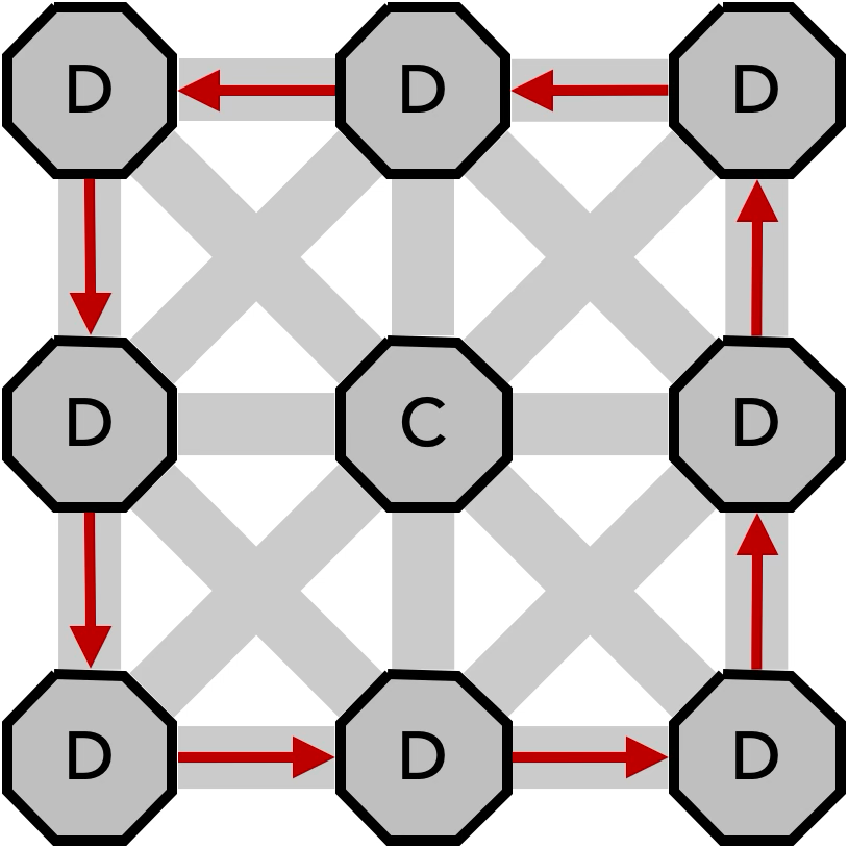
\includegraphics[width=\linewidth,trim=0mm 0mm 0mm 0mm, clip]{../../FIGURES/3x3-anticlockwise.pdf} % Trim is l b r t
  \caption{Race-Free Anticlockwise }
    \vspace{10pt}
\end{marginfigure}

Once the cell has discovered it's local environment, it may establish packet clocks. These are ANTs, which go out with a pre-defined pattern, to return events the cell on a \emph{periodic} basis.  Because there is no \emph{background} of time, this system will create events, which are guaranteed to occur without race conditions, but will catastrophically fail if there are an broken links around the circuit.

 \begin{marginfigure}
        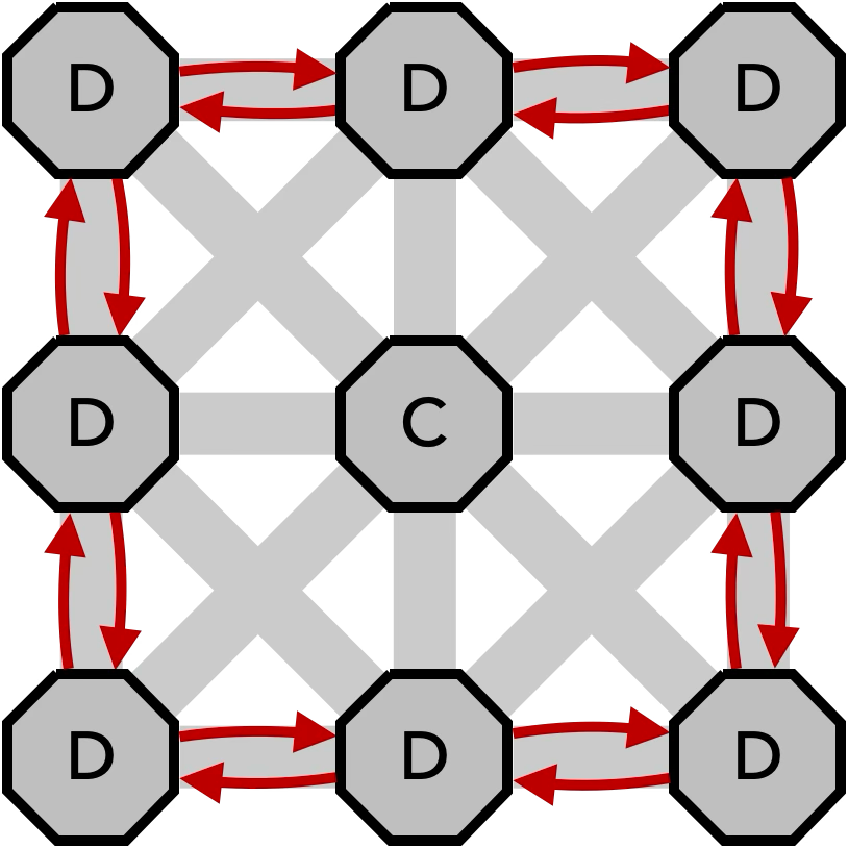
\includegraphics[width=\linewidth,trim=0mm 0mm 0mm 0mm, clip]{../../FIGURES/3x3-bothways.pdf} % Trim is l b r t
  \caption{2 Circulating Race-free tokens }
    \vspace{10pt}
\end{marginfigure}

Packets clocks may be initiated around  the closest (one-hop) cell tiles, next closest (two-hop) tiles, furthest (three-hop) tiles. Atomicity 

% FROM Spec Document SPREADSHEET-GVM copy.numbers
\subsection{ANT Specification Building a Compass Clock}
8 physical ports per cell. 
Inactive ports may be:
\begin{itemize}
\item Failed (out of service)
\item Standby, ready to go
\item Off, saving energy
\end{itemize}

\subsection{ANT Specification: Counter Circulating Race-Free ANTS}

C (Carol, Charlie, Coordinator, Chief) may initiate clockwise, counter-clockwise, and/or both at once. Each is exploring the health of the connectivity local to the center cell. This is what ANT Algorithms (source routed, or random) tokens. 



Ports at edge of mesh connected back to same cell on a different port to traverse routing table 2nd time to create  virtual cut-through torus.

If the ANT gets blocked, and either runs out of hopcout resource, it does `reverse path forwarding' back to the C CELL. and reports what it finds. It can either carry all its state in the packet, or (ror BEEs), clean up on its way and erase its footprints in the CELLs it visited.


\subsection{7 x 7 Nodes Packet Clock}
\marginnote{}

 \begin{marginfigure}
        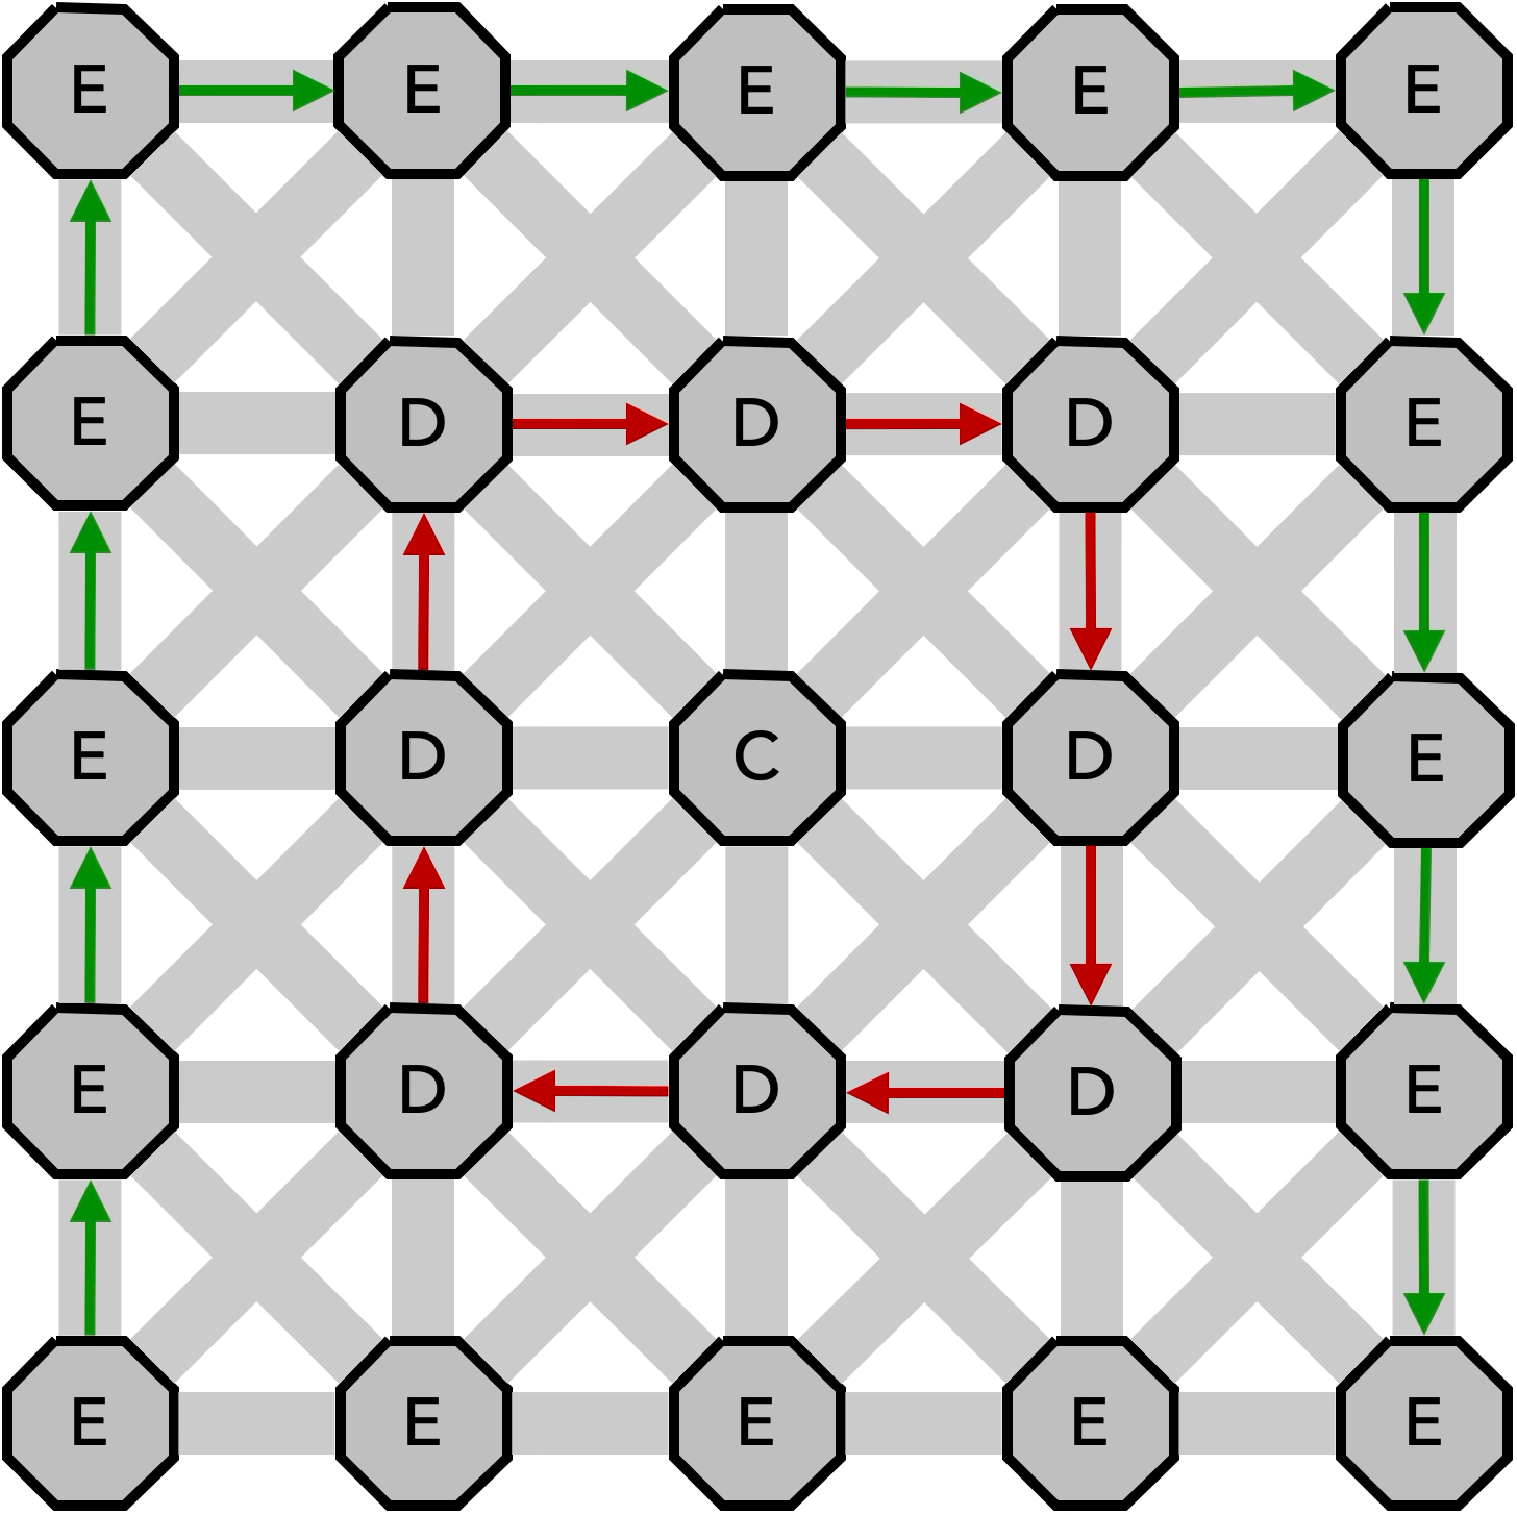
\includegraphics[width=\linewidth,trim=0mm 0mm 0mm 0mm, clip]{../../FIGURES/5x5-clock.pdf} % Trim is l b r t
  \caption{Green Packet Rateless Clock}
    \vspace{20pt}
\end{marginfigure}

\section{Beyond Packet Clocks}

Packet clocks don't scale (they are not intended to). Instead, they provide circulating logical loops \cite{Logical Clocks}.  The local system policy will establish the radius limit for local exploration. Everything beyond that is in the domain of the BEE scouts .

Packet clocks can circulate at any physical hop distance. The one-hop agents are described above.  The two figures on the right show an example of an ANT which goes two hops, or three hops, before the ANT turns left or right.  This give a CELL the opportunity to explore larger hop distances from the coordinator

\section{Packet Clocks in Larger Tiles}

 \begin{marginfigure}
        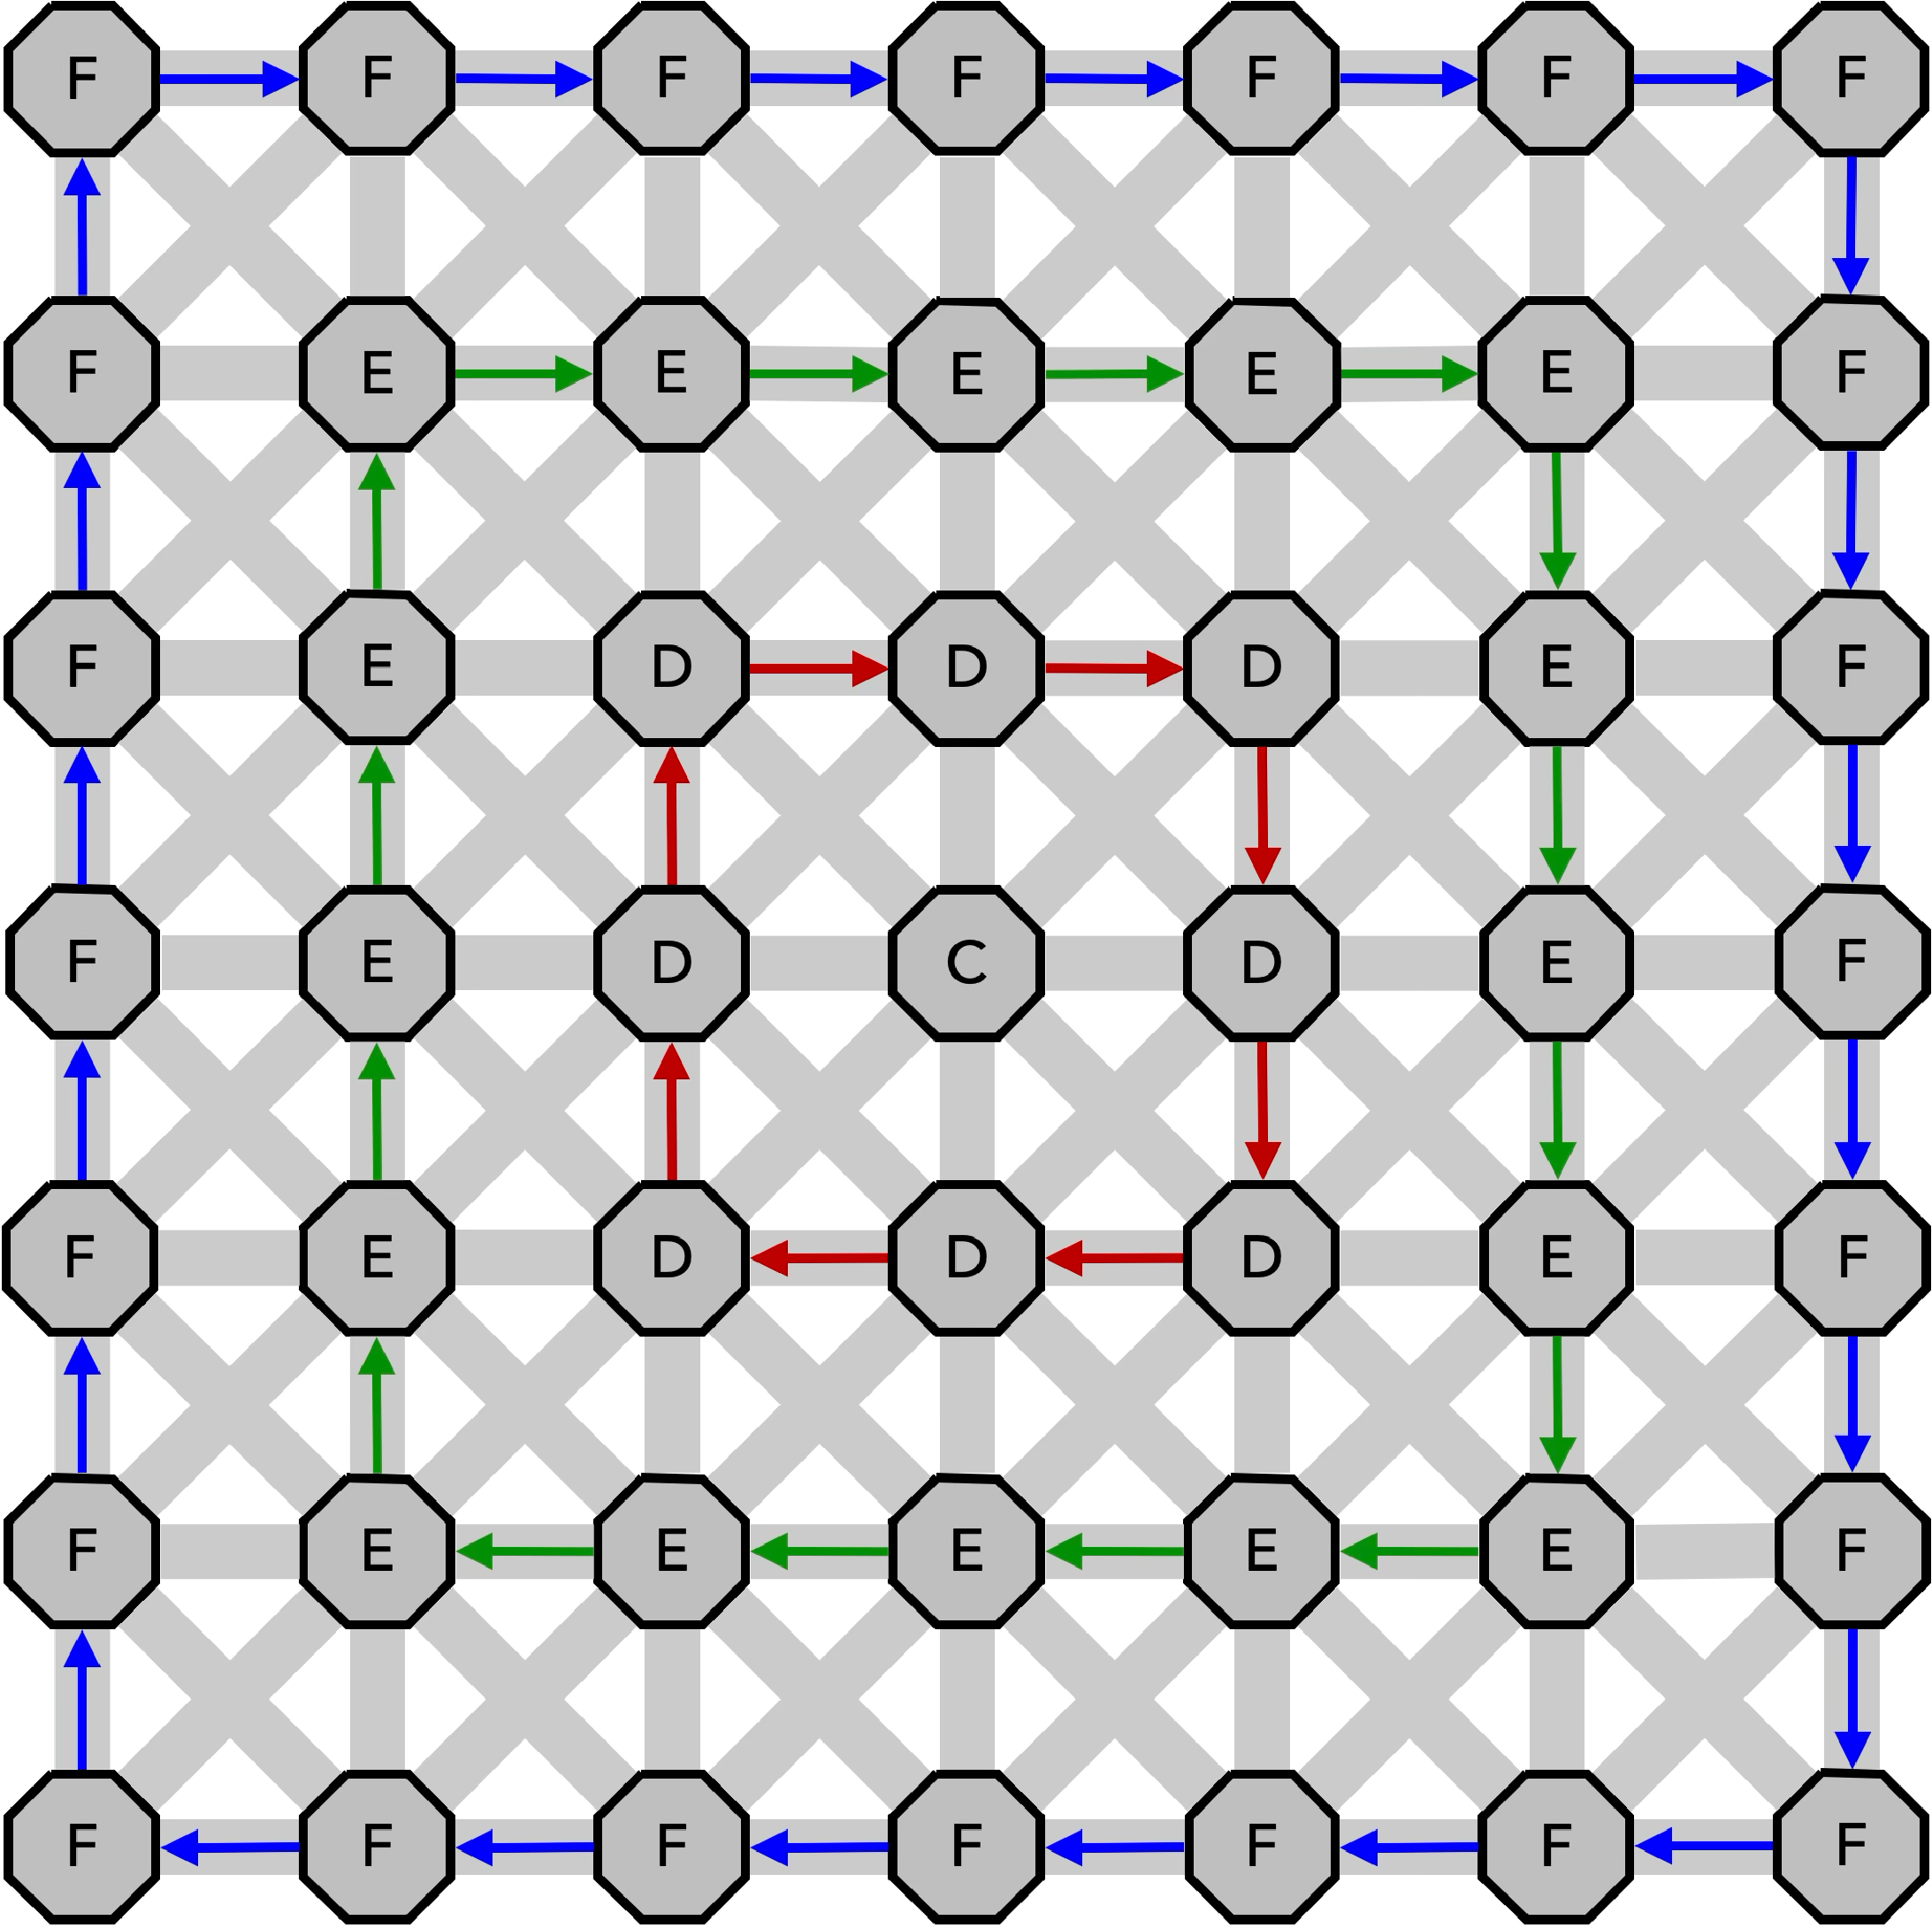
\includegraphics[width=\linewidth,trim=0mm 0mm 0mm 0mm, clip]{../../FIGURES/7x7-clock.pdf} % Trim is l b r t
  \caption{3rd-hop circular packet clocks. Blue Links Complete}
    \vspace{20pt}
\end{marginfigure}

\subsection{BEE scouts}

BEE Scouts explore the boundaries of their environment.  The are emitted by the Coordinator, and travel as far as they can in ONE direction, \texttt{\{dn,ne,de, se, ds, sw, dw, nw\}}, and then \emph{return on the reciprocal path (Compass-Point vector direction)} to inform the hive (root) what they discovered, so the root can build it's model of the topology, and Edge resources to perform their function. 

\subsection{N x N Nodes Packet Search Rays (BEEs)}

BEEs  are radial distance scouting agents. Single packets that go in only one direction, and when they reach the end (extremities of the Cellular interconnect) they execute a reverse path forwarding algorithm, collecting knowledge on their way, delivering this knowledge back to the root, whose agent  uses the returned information to build it's model of it's topology and available resources to offer `services' to the applications.

These don't have to be square, or rectangular. BEE algorithms work on any arbitrary Topology.

 \begin{marginfigure}
        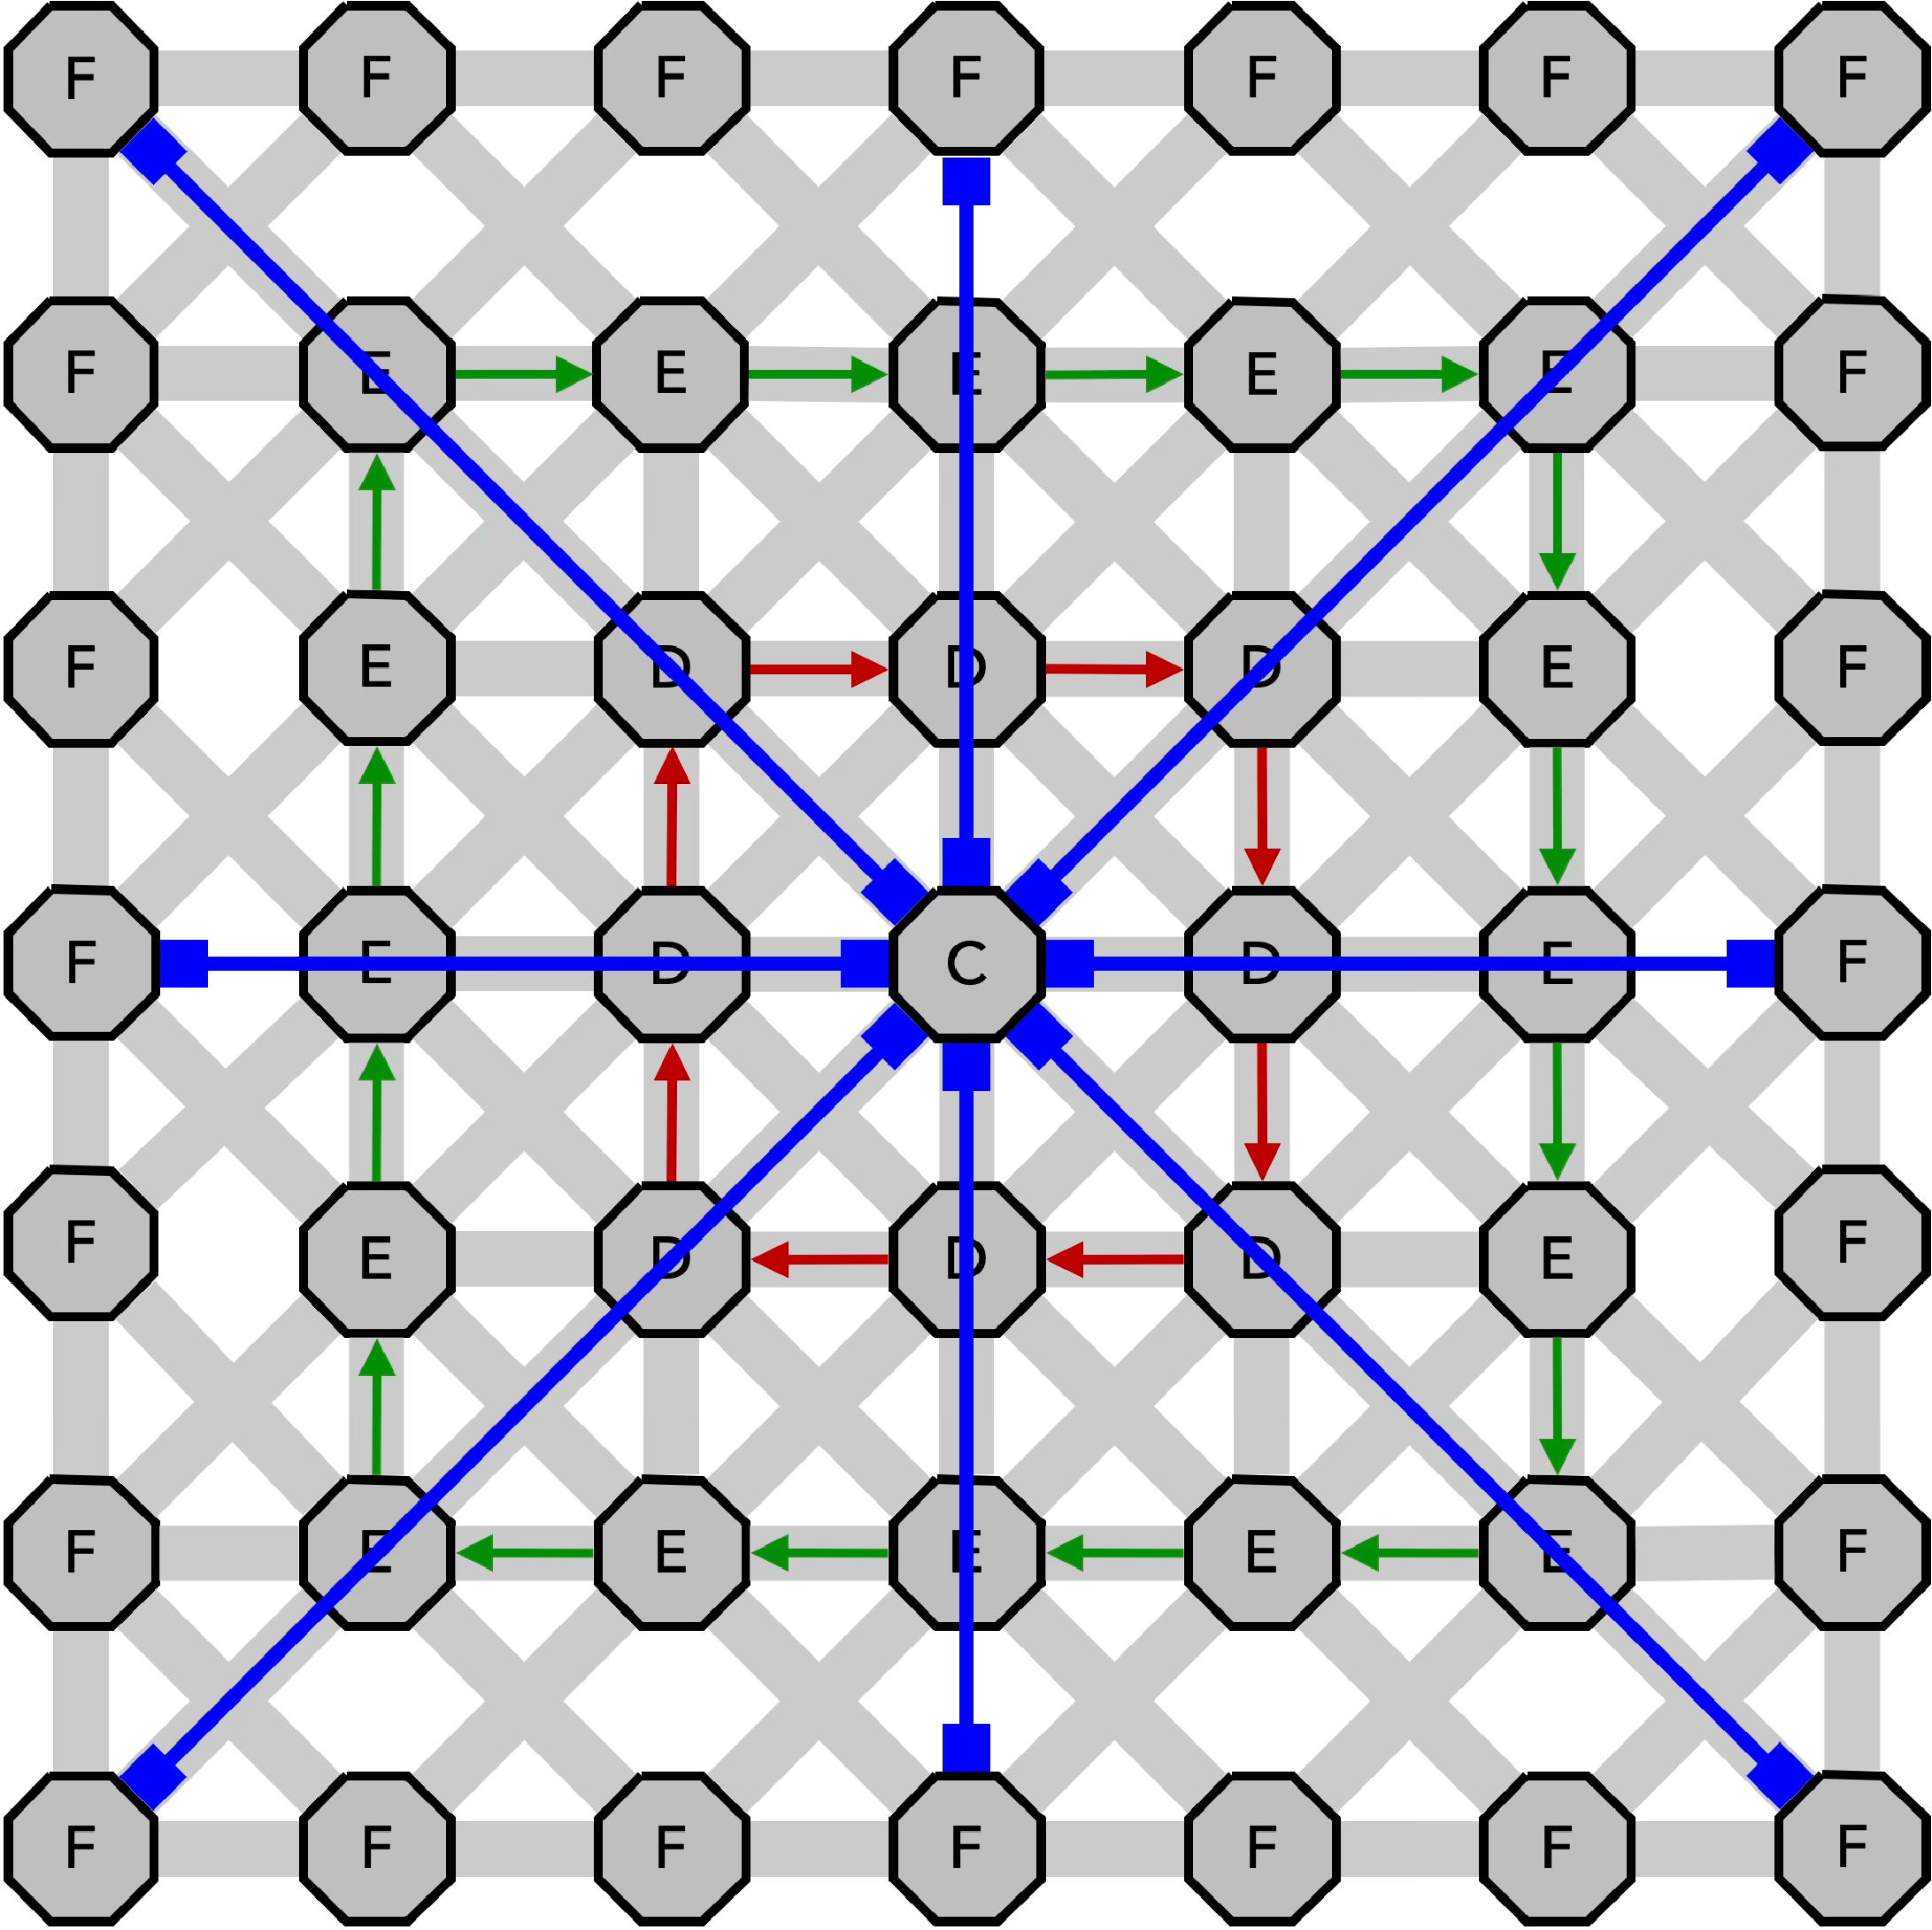
\includegraphics[width=\linewidth,trim=0mm 0mm 0mm 0mm, clip]{../../FIGURES/7x7-rays.pdf} % Trim is l b r t
  \caption{BEE Algorithms explore beyond ANT algorithms}
    \vspace{20pt}
\end{marginfigure}

Radial (Ray) source-routed scouts have two parameters (a) which port they go out on, and continue indefinitely until they reach a boundary (or exhaust their hop count resource). And then they return along exactly the same path, accumulating knowledge of the CELLS on their way (e.g. properties of the cell, do they have a CPU, a GPU, an IPU, or QPU?).  Most Bees make it back home to the nest (C) but it is also possible for a failure to occur between the outbound BEE and the homebound BEE. In which case the packet try's to make it's way to `Lost and Found', the control structures identified by the Coordinator to provide GEV notification of failures.  Lost and Found is most likely to be discovered by the one or more of the BEEs. Edge nodes (on the corners of the interconnect), will always be able to `find' Lost and Found (and other external control paths controlled by monitoring or configuration LOGICAL Administrator Agentss ) with a `due north or south'  \texttt{dn,ds}, `due-east or west' \texttt{de,dw} BEE Scout. 




\section{Local decisions and emergent global organization}

\begin{itemize}
\item Scouting/Discovery Phase: Biologically inspired methods (e.g., ant-colony-inspired or pheromone-based algorithms) often employ “scout” packets or “explorer” agents that roam the network. These scouts collect local congestion or path-quality information and deposit some form of “trail” (akin to pheromones).
\item Emergent Routing Table Updates: Each router or switch updates local routing information (sometimes called a local “pheromone table”). Over time, paths that prove consistently ``good'' get reinforced; less efficient paths fade. This local, probabilistic approach can converge on globally efficient routes with no central coordination.
\end{itemize}

\subsection{Relevance to On-Chip or 2D Mesh Topologies}

\begin{itemize}
\item Local Compass Directions: In a regular mesh (e.g., 2D grid) or torus, each router has up to 4 (N, E, S, W) or 8 ports (adding NW, NE, SW, SE). A biologically inspired algorithm can treat each output port as a possible ``direction of travel.''
\item Natural Fit for Scouting: The local directional structure matches how “ants” or “foraging agents” might look around in each direction, choosing a route based on local pheromone levels (akin to local congestion or link utilization).
\end{itemize}

Thus, the scouting/discovery mechanism is all about gathering local ``pathworthiness'' data and then directing future traffic toward better routes—exactly how a local compass-based system can easily be integrated.

\subsection{Bufferless (Hot-Potato) Routing}

\begin{itemize}
\item No Packet Buffers (or Very Limited Buffers): In a bufferless architecture, every router typically either immediately forwards or deflects each incoming packet. Packets cannot wait in large queues when an output port is congested.
\item Hot-Potato / Deflection Character: When the preferred output port is unavailable, the packet is sent out of a different (less ideal) port—``hot-potato'' style—rather than being buffered.
\end{itemize}

\subsection{Connection with Biologically Inspired Approaches}
\begin{itemize}
\item Continuous Movement: Biologically inspired scouts are already designed to wander and discover; in a bufferless system, “wandering” (via deflections) is also central. This synergy means a router can apply a heuristic (like a pheromone table) to pick the “best available port” quickly, but if that port is busy, the packet must choose an alternate direction.
\item Adaptive Reinforcement Over Time: In a bufferless design, a packet cannot linger while waiting for the optimal output. However, local “pheromone” or “congestion” metrics can still help route the majority of packets down better ports more often. Over time, high-traffic edges might become less appealing, guiding packets to less-congested directions.
\end{itemize}

\subsection{Deflection Routing}

\begin{itemize}
\item Forced Misrouting / Deflection: If the desired or minimal-distance output port cannot be taken (due to contention), the router picks another output. The packet may travel away from its ultimate destination (a “deflection”), but eventually, it should be re-routed back on track.
\item Common in Low- or No-Buffer Architectures: Deflection routing is one way to handle resource contention when buffer space is unavailable.
\end{itemize}
%
\subsection{Tying It Back to the Compass Ports (N, E, S, W, NW, NE, SW, SE)}
%
\begin{itemize}
\item Local Prioritization: In an 8-port (or 4-port) router, one can define a strict or heuristic priority among the directions. For example, a packet traveling generally “north-east” might prefer the N or E port if free; if both are busy, it might deflect NE, or in the worst case, deflect NW or SE.
\item Biologically Inspired Ranking: The “pheromone” concept can be used to rank the output directions. The highest “pheromone” port is tried first, then so on down the rank. This effectively merges a local heuristic (pheromone) with forced deflection for whichever ports remain free.
\end{itemize}

In practice, such a scheme allows packets to “scout” and reinforce certain directions while still ensuring that they never have to wait for a blocked port.

\subsection{Example Flow in an 8-Port Router}

\begin{enumerate}
\item		Receive a Packet coming in from, say, the south port.
\item		Look Up Destination (or partial coordinate heading). For instance, the packet is trying to reach a node in the north-east region, so N or E might be favored.
\item		Check Local “Pheromone” or Routing Table: Suppose the local pheromone table says port NE is the best guess based on past traffic patterns.
\item		If NE Port Is Free: Forward the packet NE.
\item		If NE Port Is Busy: Check next best local direction (N, E, or NW/SE fallback).
\item		If All Preferred Ports Are Busy: Packet is deflected to any open port (could be even SW in the worst case).
\item		Local Table Update: The router sees how that choice ended up affecting the packet (if it eventually left the region quickly or ended up in a congested area). Over time, these experiences feed back into local pheromone levels.
\end{enumerate}

Despite the forced misrouting (deflections), the biologically inspired feedback approach often keeps net throughput healthy and tries to avoid systematic congestion ``hot spots.''

\subsection{Connection with the Literature}%and Further Reading

\begin{enumerate}
\item 	1.	Hot-Potato Routing (Deflection Routing):
	\begin{itemize}
	\item Baran, P. (1962). On Distributed Communications Networks. IEEE Transactions on Communications. (Early ideas of “hot-potato” and distributed routing).
	\item Dally, W., \& Towles, B. (2004). Principles and Practices of Interconnection Networks. (Excellent overview of deflection routing in modern network design).
 	\end{itemize}

\item 	2.	Biologically Inspired / Ant-Based Routing:
	\begin{itemize}
	\item Di Caro, G. A., \& Dorigo, M. (1997). AntNet: Distributed stigmergetic control for communications networks. Journal of Artificial Intelligence Research.
	\item Schoonderwoerd, R., Holland, O., Bruten, J., \& Rothkrantz, L. (1996). Ant-based load balancing in telecommunications networks. Adaptive Behavior.
	\end{itemize}
\item	3.	Network-on-Chip with Deflection/Bufferless Approaches:
	\begin{itemize}
	\item Moraes, F. et al. (2004). A Low Area Overhead Packet-switched Network on Chip: Architecture and Prototyping. SBCCI.
	\item Fallin, C., et al. (2012). CHIPPER: A Low-Complexity Bufferless Deflection Router. HPCA.
	\end{itemize}
\end{enumerate}

These resources flesh out how bufferless or deflection routing is implemented (especially in on-chip contexts) and how biologically inspired heuristics can be adapted to local, minimal-knowledge scouting decisions.

\subsection{Concluding Remarks}

\begin{itemize}
\item Shared Tenets: Both biologically inspired scouting and deflection-based, bufferless routing rest on local decision making. In biologically inspired schemes, scouting packets “discover” or “reinforce” certain paths. In deflection routing, each router makes a quick (local) decision when a preferred port is blocked, forcing packets to keep moving.
\item Complementary Mechanics: Because biologically inspired “pheromone” updates naturally reflect congestion and path usage, they integrate well with a bufferless or deflection style—turning forced misroutes into valuable “exploration” signals that feed back into local heuristics.
\item Directional Routing: The presence of N, S, E, W (plus diagonals) simply defines how many possible local moves each node (router) can attempt. In 2D meshes or tori, these directions make for a convenient coordinate system that parallels how ants (or other scouts) might sense local gradients or pheromone intensities in each of eight compass directions.
\end{itemize}

Overall, if we combine a scouting mechanism (to adaptively find neighbors and good routes) with deflection routing (to handle buffer constraints or high contention), we get a dynamic, emergent routing system in which packets flow continuously and local updates shape global traffic patterns in a self-organizing fashion.

All this happens without the need for Source/Destination Addresses, which present severe security problems by exposing the ``identity" of nodes making them vulnerable to attack.